蒲俊才的博士论文\cite{pu-thesis}, 使用的理论框架为对 physics-informed neural network(简称 PINN) 进行改进, 为此我们需要先简要了解一下M. Raissi, P. Perdikaris 和 G.E. Karniadakis 的 PINN 模型\cite{PINN}
\begin{remark}
    如无特别声明, 本文认为神经网络, 网络, 模型是一个东西, 且混用可能机器学习和深度学习, 但本文只有深度学习. 
\end{remark}

\section{背景介绍}
在正式开始之前, 需要解释一下基础名词, 这一部分比较简单, 没有什么比较难理解的知识. 实际上神经网络也没什么难理解的, 主要是算法实现和算力限制. 
\begin{definition}{万能拟合定律}
    如果有足够的多数据, 足够多的网络层和神经元, 可以近似任意函数, 解决任何问题. 即通用人工智能(Artificial general intelligence, 简称 AGI). 
\end{definition}

\subsection{神经网络}
虽然前面说了有 PINN, 但它仍然是神经网络的一种, 原理如下图 \ref{nn-diagram} 所示. 
\begin{figure}
    \centering
    \begin{tikzpicture}[]
        \foreach \y in {1,...,2}
            \node[Node,] (I\y) at (0,17.5pt-\y*35pt) {$In_\y$};
        \foreach \y in {1,...,4}
            \node[Node,] (H1\y) at (80pt,52.5pt-\y*35pt) {$z^{(1)}_\y$};\foreach \dest in {1,...,4}
            \foreach \source in {1,...,2}
                \draw[Arrow] (H1\dest) edge (I\source);
    
        \foreach \y in {1,...,4}
            \node[Node,] (H2\y) at (160pt,52.5pt-\y*35pt) {$z^{(2)}_\y$};\foreach \dest in {1,...,4}
            \foreach \source in {1,...,4}
                \draw[Arrow] (H2\dest) edge (H1\source);
    
        \foreach \y in {1,...,2}
            \node[Node,] (O\y) at (240pt,17.5pt-\y*35pt) {$Out_\y$};\foreach \dest in {1,...,2}
            \foreach \source in {1,...,4}
                \draw[Arrow] (O\dest) edge (H2\source);
    
        \node[Tittle, above of=I1]  at (I1 |- H11) {Input};
        \node[Tittle, above of=H11]  at (H11 |- H21) {Hidden 1};
        \node[Tittle, above of=H21]  at (H21 |- H21) {Hidden 2};
        \node[Tittle, above of=O1]  at (O1 |- H21) {Output};
    \end{tikzpicture}
    \caption{神经网络示意图}
    \label{nn-diagram}
\end{figure}
\begin{definition}
    神经网络最左侧称为输入层, 最右侧称为输出层, 其余为隐藏层. 每层神经网络之间存在偏置 $ b^{(k)} $, 权重因子($w_{ij}^{(k)}$) 输入信号 $ x $ 和激活函数 $ \sigma $.
    
    如果我们记为 $w_{ij}^{(k)}$ 第 k 层第 j 个神经元指向第 k+1 层第 i 个神经元, 并假设 k 层有 n 个神经元, 则 
    \begin{equation}
        \begin{aligned}
         a_{j}^{(k+1)} &= b_{j}^{(k)} + \sum_{i=1}^{n}w_{ij}^{(k)}z_{i}^{(k)} \\
         z_{i}^{(k)} &= h(a_{j}^{(k)})           
        \end{aligned}
    \end{equation}
    其中偏置和激活函数是需要决定的, 权重因子 $ w_{ij}^{(k)} $ 是给定初值, 网络自动更新取得最优值. 

    这样的话, 如果第 k 层的矩阵综合起来记为 $ W^{(k)} $, 就会有
    \begin{equation} W^{(k)} = 
        \begin{pmatrix}
            W_{11}^{(k)} &  W_{12}^{(k)} & \cdots & W_{1n}^{(k)} \\
            W_{21}^{(k)} &  W_{22}^{(k)} & \cdots & W_{2n}^{(k)} \\
            \vdots & \vdots & \ddots & \vdots \\
            W_{n1}^{(k)} &  W_{n2}^{(k)} & \cdots & W_{nn}^{(k)}
        \end{pmatrix}
    \end{equation}
    则第 k 个网络层的计算可以视为 
    \begin{equation}
        \mathcal{L}_k = W^{(k)}\textbf{x}^{(d-1)} + \textbf{b}^{(k)}
    \end{equation}
    整个网络的的计算可以视为
    \begin{equation}
             Output = \big( \mathcal{L}_d \circ \sigma \circ \mathcal{L}_{d-1} \circ \sigma \cdots \circ \mathcal{L}_{2} \circ \sigma \circ \mathcal{L}_{1} \big) (\textbf{x})    
    \end{equation}
\end{definition}


\begin{remark}
    输入层为第 0 层, 网络的层数 = 隐藏层+输出层. (因为必须有计算才算层数, 输入层仅仅导入数据, 所以不算层数.)
\end{remark}
\begin{remark}
    实际上神经网络的每一层应该是如图 \ref{nn-node-diagram}. 此外现在还有 Batch-normalization 层, Residual 层。
    \begin{figure}
        \centering
        \begin{tikzpicture}[x=0.75pt, y=0.75pt, scale=1]
            % Input nodes
            \node[Node] (input3) at (50, 100) {$z_2$};
            \node[Node] (input2) at (50, 150) {$z_1$};
            \node[Node] (input1) at (50, 200) {$1$};            
            % Weighted sum node
            \node[Node] (sum) at (150, 150) {$a_{j}^{(k)}$};            
            % Output node
            \node[Node] (output1) at (220, 150) {$z_{j}^{(k)}$};
            \node[Node] (output2) at (320, 150) {$a_{j}^{(k+1)}$};           
            % Connections
            \draw[Arrow] (sum) -- (input1) node[midway, above] {$b_{j}^{(k)}$};
            \draw[Arrow] (sum) -- (input2) node[midway, above] {$w_{j1}^{(k)}$};
            \draw[Arrow] (sum) -- (input3) node[midway, above] {$w_{j2}^{(k)}$};
            \draw[Arrow] (output1) -- (sum) node[midway, above] {$\sigma$};
            \draw[Arrow] (output2) -- (output1) node[midway, above] {$w_{ij}^{(k)}$};
            % Circle around sum and output
            \node[groupcircle, fit={(sum) (output1)}] {};
        \end{tikzpicture}
        \caption{实际节点原理图, 以 $ z_{j}^{(k)} $ 为例}
        \label{nn-node-diagram}
    \end{figure}
\end{remark}
\begin{remark}
    Lu Zhou 和 Pu Hongming 的论文 \cite{lu2017expressivepowerneuralnetworks} 论证了神经网络层数和神经元的关系, 即浅层网络可以通过增加神经元的方式达到和深层网络差不多的效果, 但是需要指数级的增加. 这也很好理解, 假设 A 是一个 10 层的网络, 每层 100 个神经元; B 是 100 层的网络, 每层 10 个神经元. 假设每个神经元花费的内存和算力相同, 那么 A 消耗的算力是 $100^{10}$, B 是 $10^{100}$. 所以对于深度学习而言, 增加网络层是比增加神经元更好的方法. 
\end{remark}

\begin{definition}
    由于数据量过小, 或者训练方法不对, 只能解决某个特殊问题, 称为过拟合(Overfitting). 
\end{definition}
\begin{remark}
    虽然深度学习的目标是 AGI, 追求泛化能力, 但是在建立模型的时候还是先追求过拟合, 然后再抑制过拟合, 追求泛化能力. 一般使用 $ \mathbb{L}_{2} $ 来抑制过拟合, 如果是特别复杂的网络, 会使用 Dropout 来抑制过拟合.  
\end{remark}

\subsection{激活函数}
激活函数一般是神经网络中激活神经元的一种非线性函数,常用 $\sigma$ 表示,一般而言神经网络每层的激活函数都相同, 唯有输出层为 Softmax 映射 (归一化), 常见的激活函数如下所示. 

首先是应用最广泛的 Sigmoid 函数和蒲的论文使用的 tanh 函数, 以及归一化的 Softmax 函数. 
\begin{equation}
    \begin{aligned}
        \text{sigmoid}(x) = \frac{1}{1+e^{-x}}, \\ 
        \tanh{(x)} = \frac{e^{x} - e^{-x}}{e^{x} + e^{-x}} \\
        \text{softmax}(a_k) = \frac{\exp a_k}{\sum_{i=1}^{n} \exp a_i}
    \end{aligned}
\end{equation} 
易见 
\begin{equation}
    \tanh(x) = 2 \text{sigmoid}(2x) - 1
\end{equation}
且他们的导函数分别为
\begin{align}\label{loss-example}
    \text{sigmoid}'(x) &= \frac{e^{-x}}{(1+e^{-x})} = \text{sigmoid}(x)(1-\text{sigmoid}(x)) \\
    \tanh '(x) &= \frac{4}{(e^x + e^{-x})^2} = \sech^{2}(x) = 1 - \tanh ^{2}(x)
\end{align}
它们的函数图像见图 (\ref{fig:Sigmoid})
\begin{figure}[htbp]
    \centering
    \begin{subfigure}{0.49\textwidth}
        \centering
        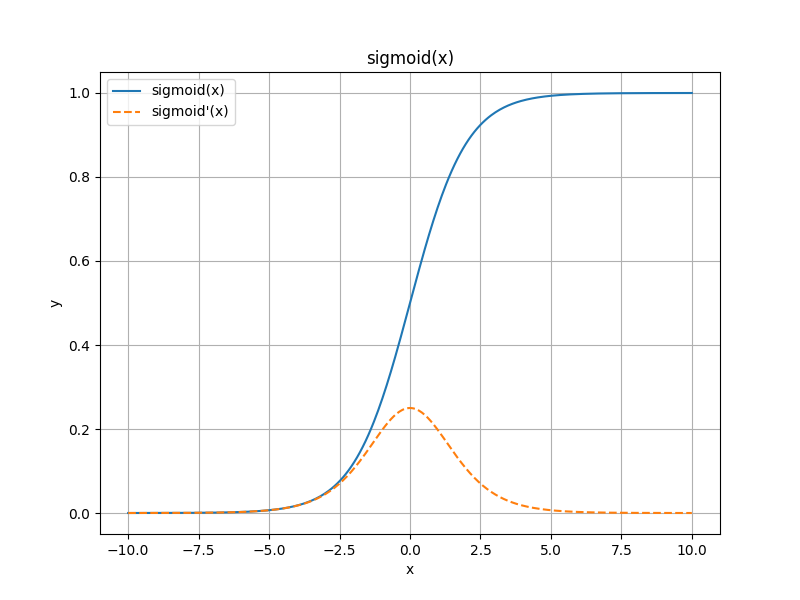
\includegraphics[width=\textwidth]{images/sigmoid.png}
        \caption{Sigmoid}
        \label{fig:sigmoid}
    \end{subfigure}
    \hfill
    \begin{subfigure}{0.49\textwidth}
        \centering
        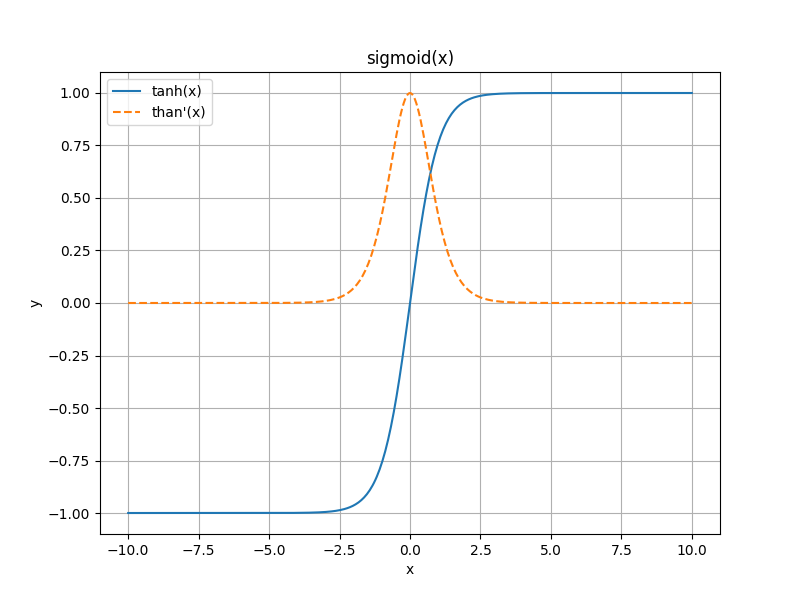
\includegraphics[width=\textwidth]{images/tanh.png}
        \caption{tanh}
        \label{fig:tanh}
    \end{subfigure}
    \caption{Sigmoid 和 tanh 函数图}
    \label{fig:Sigmoid}
\end{figure}

Sigmoid 函数和 tanh 函数在两端都比较平坦,即其对应的导数趋向于 0. 当使用这些饱和激活函数(如sigmoid)的神经网络进行反向传播时,那些输出值在0或1附近的神经元梯度几乎为0, 这些神经元通常被称为饱和神经元. 相应地, 这些神经元的权重将无法得到更新, 且与之相连的神经元的权重更新也非常缓慢. 在某些情况下, 最终训练好的网络会收敛到一个很差的局部极小值. 这就是所谓的梯度消失问题.
\begin{remark}
    $ \tanh $ 比 $ sigmoid $ 更好的点在于它关于原点中心对称, 这种良好的对称性使其对网络训练有极好的效果
\end{remark}

此外, sigmoid 函数和 tanh 函数在计算过程中都使用了指数函数,这样的函数运算计算开销很大. 一些其它函数,如softsign等被提出用于替代tanh函数. 但是, 这些函数或多或少仍然存在上面所说的梯度消失等问题. 因此, 我们想要一种既是非线性, 又处处可微, 而且在无穷远处导数为 0 的函数.  

\subsection{损失函数}
损失函数用来衡量网络性能的 ``恶劣程度'', 所以损失函数越小越好. 常见的损失函数有均方误差(mean squared error, 简称 MSE) 平方和误差(Error Sum of Squares, 简称 SSE)和交叉熵误差(cross entropy error, 简称 CEE)
\begin{equation}
    \begin{aligned}
        MSE &= \frac{1}{n} \sum_{i=1}^{n} (y_i - \hat{y}_i)^2 \\
        CEE &= - \sum_{i=1}^{n} \big[ y_i \ln(\hat{y}_i) + (1 - y_i) \ln(1 - \hat{y}_i) \big]
    \end{aligned}
\end{equation}
其中 $ y_i $ 是实际值,$ \hat{y}_i $ 是预测值,$ n $ 是样本数量. 
这里面 MSE 一般用作隐藏层(Affine 层)的损失函数, CEE 一般用作输出层损失函数, 使得反向传播的结果``非常简单''. 
一般而言, 想要达到 95\% 以上的精度, 需要损失函数在 $ 10^{-4} $ 的量级. 

\begin{remark}
    这里大致介绍一下反应网络的几个指标 
    \begin{enumerate}
        \item Loss: 用来训练网络, 使其达到好结果
        \item $ \mathbb{L}_{2} $: 抑制过拟合, 一般比 Loss 大一两个量级
        \item 正确率: 网络预测结果/真实结果
        \item 精度: 最小``步长'', 如 1e-4, 1e-8 等.
    \end{enumerate}
\end{remark}
\subsection{反向传播算法和自动微分}
如果说前向 (前馈) 传播是由因及果的话, 那反向传播就是由果及因. 前向传播阶段将训练数据输入网络,经过一系列的矩阵乘法和非线性变换操作,得到最终的预测结果. 反向传播阶段根据预测结果与真实结果之间的误差,利用反向自动微分和链式法则,从后往前逐层计算每个神经元的误差贡献,以此更新神经元的权重. 

在讲反向传播之前, 我们还需要先简要了解一下自动微分和它的缺点. 我们都知道 
\begin{definition}函数 $ f $ 导数的定义是: 
    \begin{equation}
        \frac{d f}{d x} = \lim_{h \to 0} \frac{ f(x + h) - f(x) }{h} 
    \end{equation}
\end{definition}

实际上计算机并不能取到无穷小, 如果我们设 $h = 10^{-10}$, 那么在 float32 类型下计算会因为精度问题输出为 0, 这时候就会出现梯度消失, 因为 float32 的精度约为 $10^{-7}$. 为此,我们常用 float64 类型来提高精度, 但它占用的内存和计算开销通常是 float32 的两倍. 在机器学习中, 由于 float32 精度已经足够, 因此通常使用 float32 类型. 当然, 我们也可以使用中心求导等方式减小误差. 为此我们选用反向传播算法, 它从原理上越过了舍入误差, 并且极大的加快了训练速度. 
\begin{remark}
    我曾经测试过这两个算法的区别, 反向传播使用 300MB, 7 min 完成推理, 数值微分直接内存跑到了 16 GB 关机了. 后来多次调整之后, 数值微分 15.5 GB 内存, 1 h 完成的项目, 反向传播只需要 227 MB, 7 min 完成.
\end{remark}

图 (\ref{fig:BP-theory}) 是误差反向传播算法的原理示意图
\begin{figure}[htbp]
    \centering
    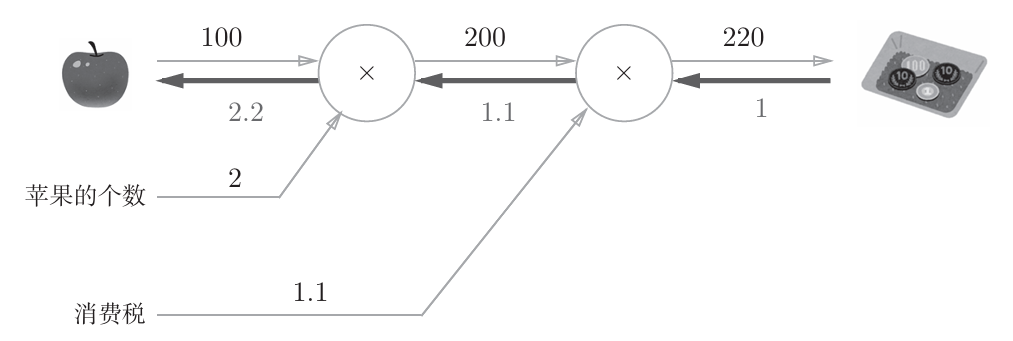
\includegraphics{images/bp-theory.png}
    \caption{反向传播原理}\label{fig:BP-theory}
\end{figure}

反向传播和常规求导不同在于, 常规求导为 $ y' = f(x) $, 反向传播使用 $ y = F(y) $ 表示, 如上面的 (\ref{loss-example}) 式, 

如果设 $ \mathbf{L} = \mathbf{W} \mathbf{x} + \mathbf{b} $, 其中  $ \sigma $ 为激活函数, 则 
\begin{equation}
    \frac{\partial \sigma}{\partial \mathbf{x}} = \mathbf{W}^{T} \cdot \frac{\partial \sigma}{\partial \mathbf{L}},  
    \quad
    \frac{\partial \sigma}{\partial \mathbf{W}} =\frac{\partial \sigma}{\partial \mathbf{L}} \cdot \mathbf{x}^{T},  
\end{equation}
\begin{remark}
    注意这里使用分子布局是为了对齐维度, 更多内容请见 \href{https://en.wikipedia.org/wiki/Matrix_calculus}{Matrix calculus}
\end{remark}
同样的, 机器学习里面的 ``梯度下降'' 也不是我们数学上的梯度下降, 而是
\begin{equation}
    x_0 \leftarrow x_0 - \eta \frac{\partial f}{\partial x_0}, \quad x_1 \leftarrow x_1 - \eta \frac{\partial f}{\partial x_1}
    \label{grad-fall}
\end{equation}
其中 $ \eta $ 表示更新量, 在神经网络的学习中, 称为学习率 (learning rate). 学习率决定在一次学习中, 应该学习多少, 以及在多大程度上更新参数. (\ref{grad-fall}) 式是表示更新一次的式子, 这个步骤会反复执行. 也就是说, 每一步都按上更新变量的值, 通过反复执行此步骤, 逐渐减小函数值. 虽然这里只展示了有两个变量时的更新过程, 但是即便增加变量的数量, 也可以通过类似的式子(各个变量的偏导数)进行更新. 学习率需要事先确定为某个值, 比如 0.01 或0.001. 然后根据训练结果逐步调整. 一般而言,这个值过大或过小, 都无法抵达一个 ``好的位置''. 一般的取值范围为 $ [10^{-3}, 10^{-2} ] $. 

而且哪怕 lr 取得比较好, 梯度法也不一定能达到最小值, 我们都知道梯度指向的是函数下降的方向, 它必然是极小值但不一定是最小值, 此外,当函数很复杂且呈扁平状时, 还会有 ``鞍点'', 这就是梯度消失. 此时学习会进入一个 (几乎) 平坦的地区, 陷入被称为“学习高原”的无法前进的停滞期。

\subsection{Batch 和 mini-Batch}
这样设想一下, 我们想要训练的数据量称为 Batch, 假设有 100 个数据, 很轻松就能直接训练完看结果如何. 但是假设有一千万乃至一亿数据, 还是一下都训练完的话, 很可能需要数天乃至数月的时间, 所以我们想要先试出来一个比较好的学习率 lr, 然后再进行训练. 所以需要抽样, 也就是 mini-Batch. 比方我们想要先抽 100 个, 那么 mini-Batch 就是 100. 

说到这里, 差不多前置知识就说完了, 总结一下, 对于深度学习, 只需要确定激活函数, 学习率和 mini-Batch(也成为超参数), 其余参数均交给网络自己决定. 

\subsection{权重初始值 与 Xavier 正则化}
接下来我们继续想办法解决梯度消失/爆炸问题. Xavier 是目前常用的正则化方法, 其基本思想是通过适当的随机初始化(一般为 Gauss 分布), 使得该层输入个数不影响每层输出的方差, 该层输出个数也不影响每层梯度的方差, 从而加快网络训练速度并提高网络训练精度. Xavier 初始化的具体实现为假设 $ W $为 $ n_{in} \times n_{out} $ 维的权重矩阵, 其中 $ n_{in}$  和 $ n_{out} $ 分别表示该层输入输出. 则 $ W $ 的初始化应该满足
\begin{equation}
    Var(M) = \frac{2}{n_{in}+n_{out}}
\end{equation}
其中Var表示方差. 蒲的论文也是用的 Xavier 正则化.
\subsection{优化器}
接下来说一下怎么更新网络信息, 寻找最小 Loss, 即优化器. 时间紧迫, 我们只说一个 Adam\cite{Adam} 优化器, 这也是目前业界主流的优化器, 它结合了 Momentum 和 Adagrad 的优点, 通过一阶和二阶矩\footnote{这里一阶和二阶矩为均值和方差}的信息来调整学习率, 提升训练速度和收敛效果. 

Adam 算法核心思想是根据历史梯度的平均值和方差来自适应地调整学习率. 具体地, 对于每个参数, Adam算法维护分别表示梯度的一阶矩和二阶矩估计的两个变量 $ \textbf{m} $ 和 $ \textbf{v} $. 这里 $ \textbf{m} $ 和 $ \textbf{v} $ 的初始值设置为 0, 在每次迭代中先计算梯度 $ g_{t} $, 然后再分别更新 $ m $ 和 $ v$, 具体过程如下
\begin{equation}
    \textbf{m}_t \leftarrow \beta_{1} \textbf{m}_{t-1} + (1-\beta_1)g_t, \quad \textbf{v}_t \leftarrow \beta_{1} \textbf{v}_{t-1} + (1-\beta_1)g_{t}^{2}
\end{equation}
其中$ \beta_1, \beta_2 $ 分别表示指数加权移动平均的衰减率 (通常取值为0.9和0.999), $ g_t $ 表示在当前迭代中计算得到的梯度. 为了减少偏差, 上述更新公式 $ m $ 和 $ v $ 的初始值都需要进行偏置修正后再来计算参数更新量, 具体表达式如下:
\begin{equation}
    \hat{m}_t \leftarrow \frac{m_t}{1 - \beta_{1}^t}, \quad 
    \hat{v}_t \leftarrow \frac{v_t}{1 - \beta_{2}^t}, \quad
    \theta_{t+1} \leftarrow \theta_t - \frac{\alpha \cdot \hat{m}_t}{\sqrt{\hat{v}_t} + \epsilon}
\end{equation}
其中 $ \eta $ 表示学习率, $ \epsilon $ 是一个很小的常数, 用于防止分母为 0 的情况发生.相比于其他算法, Adam 算法具有以下优点
\begin{itemize}
    \item 自适应学习率: Adam 对每个参数采用不同的学习率, 自适应地调整学习率。
    \item 收敛性好: 使用了动量项\footnote{这里的动量项也不是物理上的动量, 而是 Momentum 项}, Adam 可以加速收敛, 减少振荡.\footnote{在计算梯度时不仅考虑当前的梯度, 还考虑历史梯度的平均值; 使用了自适应的二阶矩估计, 即在计算梯度时不仅考虑历史梯度和当前梯度的平均值, 而且考虑了二阶矩的平均值.}
    \item 适合稀疏梯度: Adam 在高维空间和稀疏数据 (如文本或图像) 上有较好表现
    \item 计算效率高: Adam 的计算效率较高, 内存需求低. 
\end{itemize}